% ICML 2025 Paper Template for Overleaf
% Auto-generated by Anonymous Research Pipeline
%
% Instructions:
% 1. Upload this folder to Overleaf
% 2. Ensure icml2025.sty is in the same directory
% 3. Compile with pdfLaTeX
%
\documentclass{article}

% ICML 2025 style
\usepackage{icml2025}

% Standard packages
\usepackage{microtype}
\usepackage{graphicx}
\usepackage{booktabs}
\usepackage{hyperref}
\usepackage{amsmath}
\usepackage{amssymb}
\usepackage{algorithm}
\usepackage{algorithmic}

% For better table formatting
\usepackage{multirow}
\usepackage{makecell}

% Bibliography
\usepackage{natbib}

% ============================================================================
% DOCUMENT METADATA
% ============================================================================

\icmltitlerunning{The Coordinate System, Not the Symmetry Group}

\begin{document}

\twocolumn[
\icmltitle{The Coordinate System, Not the Symmetry Group: Graph-Based SSL for Cross-Architecture Weight Space Transfer}

\icmlsetsymbol{equal}{*}

\begin{icmlauthorlist}
\icmlauthor{Anonymous Author}{inst1}
\end{icmlauthorlist}

\icmlaffiliation{inst1}{Anonymous Institution}

\icmlcorrespondingauthor{Anonymous Author}{anonymous@institution.edu}

\icmlkeywords{Machine Learning, ICML, weight space learning, graph neural networks, self-supervised learning, cross-architecture transfer}

\vskip 0.3in
]

\printAffiliationsAndNotice{}

% ============================================================================
% ABSTRACT
% ============================================================================

\begin{abstract}
Predicting properties of trained neural networks from their weights --- model zoo analysis ---
typically assumes that test models share the same architecture as training models.
When this assumption breaks, flat tokenization methods collapse:
we show that SANE, the current state of the art for within-architecture weight-space SSL,
maps all ViT inputs to near-identical latent codes after training on CNN checkpoints,
achieving $R^2 = 0.072$ (near-chance) on 53 held-out ViT-S/16 ImageNet checkpoints.
We propose that the root cause is the \emph{representation substrate}, not the learning algorithm:
flat weight tokenization discards the relational graph structure that is consistent across architecture families.
We train a permutation-equivariant graph SSL encoder on MLP/CNN model zoos
and demonstrate zero-shot cross-architecture transfer to ViT property prediction,
achieving $R^2 = 0.231$ versus SANE's $R^2 = 0.072$ --- a $3\times$ improvement ---
without any ViT training data.
Counterintuitively, adding scale equivariance to the symmetry group hurts rather than helps ---
we attribute this to a \emph{LayerNorm gauge-fixing hypothesis}:
LayerNorm eliminates the scale degree of freedom that scale equivariance is designed to handle,
making scale invariance an incorrect inductive bias for ViT weight encoding.
These results suggest that the coordinate system (computational graph schema)
matters more than the symmetry group for cross-architecture weight representation learning.

\end{abstract}

% ============================================================================
% MAIN CONTENT
% ============================================================================

\section{Introduction}

A neural network encoder trained exclusively on small MLP and CNN checkpoints ---
without ever seeing a transformer during training ---
can predict ViT model accuracy three times better than the state-of-the-art
weight-space self-supervised learning method.
The key is not the symmetry group. It is the coordinate system.

This result emerges from a question at the intersection of two research agendas:
\emph{how do we represent the weights of a neural network in a way that is useful?}
and \emph{can representations learned from one family of architectures transfer to another?}
These questions matter because model zoo analysis --- predicting properties of arbitrary trained
networks without retraining --- is increasingly important for model selection,
architecture search, and continual learning at scale.
Yet existing methods silently assume that the test models come from the same architecture
family as the training models.
When that assumption breaks, they fail.

We find that it breaks in a specific, diagnosable way.
The SANE method~\cite{Schurholt2024Towards} ---
which achieves strong performance ($R^2 = 0.72$) in its intended within-architecture setting ---
represents each neural network as a flattened sequence of weight scalars,
agnostic to network topology.
When presented with ViT checkpoints after training on MLP/CNN checkpoints,
SANE maps all inputs to near-identical latent codes ($\text{std} \approx 0.0014$).
The representation has collapsed: every ViT model looks the same to the encoder,
regardless of its accuracy.
This is not a degradation in quality; it is a fundamental failure of the representation
substrate under cross-architecture distribution shift.

The failure mode reveals the solution.
What flat tokenization discards is the \emph{relational structure} of a neural network ---
the computational graph of neurons connected by scalar weights.
This structure is architecture-agnostic: a ViT attention projection layer,
a CNN convolutional filter, and an MLP linear layer are all, at bottom,
directed graphs of neurons and edges.
If we encode weights \emph{in terms of their graph structure} rather than as flat sequences,
the encoder sees a consistent vocabulary across architectures.
A permutation-equivariant graph neural network trained on this representation
can process ViT weight graphs even though it was trained only on CNN weight graphs,
because the graph schema is the same.

Our key insight:
\textbf{the directed computational graph schema (node=neuron, edge=weight)
provides a universal weight-space coordinate system that enables SSL representations
trained on MLP/CNN model zoos to generalize directly to ViT model zoo property prediction
without any ViT training data.}
The specific symmetry group --- whether to enforce scale equivariance in addition to
permutation equivariance --- turns out to be secondary.
Counter to predictions from supervised same-architecture
settings~\cite{Kalogeropoulos2024Scale},
scale+permutation equivariance (EquiSSL) achieves $R^2 = 0.185$ on held-out ViT models
while permutation-only equivariance (EquiSSL-perm) achieves $R^2 = 0.231$ ---
a reversal of the expected ordering.
We hypothesize that LayerNorm in ViT architectures eliminates the scale degree of freedom
that scale equivariance targets, making scale invariance an incorrect inductive bias for
ViT weight encoding (see Section~\ref{sec:layernorm}).
This LayerNorm gauge-fixing hypothesis is empirically motivated;
independent theoretical treatment, if verified, would provide additional support.

This paper makes the following contributions:

\textbf{(1)} We identify and characterize the latent collapse failure mode of flat tokenization
under cross-architecture SSL.
On 53 real ViT-S/16 ImageNet checkpoints, SANE achieves $R^2 = 0.072$ --- near-chance
for regression --- with latent variance $\text{std} \approx 0.0014$ indicating collapsed
representations.
Note that SANE is not a generally poor method --- it achieves $R^2 = 0.72$ in its intended
within-architecture setting; the $R^2 = 0.072$ reflects the cross-architecture distribution
shift failure mode specifically.

\textbf{(2)} We demonstrate that graph-based SSL with permutation equivariance achieves meaningful
cross-architecture transfer without target-domain training data.
EquiSSL-perm achieves $R^2 = 0.231$ on 53 held-out ViT-S/16 models ---
a ${\sim}220\%$ improvement over SANE, providing initial proof-of-concept evidence for
cross-architecture SSL transfer.

\textbf{(3)} We discover that scale equivariance does not improve over permutation-only equivariance
for ViT cross-architecture transfer, providing empirical support for the LayerNorm
gauge-fixing hypothesis.
EquiSSL achieves $R^2 = 0.185$ (ablation evaluation, Table~\ref{tab:ablation}),
underperforming EquiSSL-perm ($R^2 = 0.327$ in the same ablation evaluation;
$R^2 = 0.231$ in the main experiment, Table~\ref{tab:main}).
The directional ordering (EquiSSL-perm $>$ EquiSSL $>$ SANE) is consistent across both
evaluations, though absolute magnitudes differ due to training duration differences.

\textbf{(4)} We diagnose why graph-based latent interpolation fails as a model editing primitive.
Latent interpolation achieves $\text{acc} = 0.100$ = exactly random chance ($1/10$ for CIFAR-10),
while weight-space averaging achieves $\text{acc} = 0.125$ ($p \approx 0$, Cohen's $d = -1.10$).
Property prediction and model generation are separable capabilities requiring architecturally
distinct decoders.

We organize the paper as follows.
Section~\ref{sec:related} surveys related work.
Section~\ref{sec:method} describes our methodology.
Section~\ref{sec:setup} details our experimental setup.
Section~\ref{sec:results} presents results.
Section~\ref{sec:discussion} discusses surprising findings, limitations, and broader implications.
Section~\ref{sec:conclusion} concludes.

\section{Related Work}
\label{sec:related}

\subsection*{Weight-Space Self-Supervised Learning}

The idea of learning representations from neural network weights ---
treating checkpoints as data --- has attracted growing attention.
Hyper-Representations~\cite{Schurholt2021Hyper} first demonstrated that training an autoencoder
on populations of neural network weights produces latent codes that recover hyperparameters,
accuracy, and generalization gap without task labels.
SANE~\cite{Schurholt2024Towards} extended this to a hierarchical transformer architecture
with contrastive SSL, achieving $R^2 = 0.72$ on heterogeneous model zoo property prediction
within its intended same-architecture setting.
Both methods use \emph{flat tokenization}: weight matrices are chunked into fixed-size tokens,
processed positionally, and aggregated ---
an approach that implicitly assumes weight token positions are comparable across networks.

This assumption holds when training and test architectures share the same layer structure.
When architectures differ substantially (e.g., MLP/CNN vs.\ ViT), flat tokenization loses meaning.
Our work identifies the consequence:
SANE's latent representations collapse to near-constant codes for cross-architecture inputs
($\text{std} \approx 0.0014$), and property prediction drops to $R^2 = 0.072$.
This is a cross-architecture distribution shift failure, not a failure of SANE as a method
in its intended domain.
The graph encoding approach we adopt directly addresses this structural mismatch.

\subsection*{Equivariant Graph Neural Networks for Weight Encoding}

A parallel research strand represents neural networks as computation graphs and uses
equivariant GNNs as encoders.
The foundational theoretical work~\cite{Navon2023Equivariant} characterized all
permutation-equivariant/invariant linear layers over weight spaces.
Neural Functional Transformers~\cite{Zhou2023Permutation} and
NF-Layers~\cite{Kofinas2024Graph} demonstrated that graph-based encoders achieve strong
performance on property prediction within a fixed architecture family.
Critically, Kofinas et al.~\cite{Kofinas2024Graph} showed that graph-based encoders can
generalize \emph{across} architecture families in the \emph{supervised} setting,
achieving $R^2 = 0.71$ on held-out CNNs after training on MLPs.
ScaleGMN~\cite{Kalogeropoulos2024Scale} extended this to include scale equivariance,
showing $+8$--$12$ $R^2$ points over permutation-only baselines in supervised same-architecture
settings.
Our work differs in two key dimensions:
(1) we operate in the \emph{self-supervised} setting; and
(2) we target \emph{cross-architecture} transfer to ViTs with LayerNorm,
which changes the benefit profile of scale equivariance.

\subsection*{Cross-Architecture Weight Representation Transfer}

The most directly related work is Ballerini et al.~\cite{Ballerini2025Weight},
who applied contrastive SSL to diverse neural radiance field architectures and demonstrated
cross-architecture property transfer without target-domain training data.
Our work generalizes this paradigm to general-purpose neural architectures
(MLPs, CNNs, ViTs) --- a broader and more architecturally diverse setting.
The ViT Model Zoo~\cite{Falk2025ModelZoo}, which provides real ViT-S/16 ImageNet
checkpoints with accuracy labels, enables evaluation of cross-architecture SSL at scale;
we use their dataset as our test set.

\subsection*{Symmetry and Normalization Layers}

The interaction between equivariance symmetry groups and neural network normalization has
received recent theoretical attention.
We hypothesize that LayerNorm in transformer architectures fixes the gauge degree of freedom
corresponding to activation scale, reducing the effective symmetry group of ViT weight spaces
to permutation-only.
Our empirical finding --- that scale equivariance \emph{hurts} ViT cross-architecture transfer ---
provides experimental support for this hypothesis.

Existing weight-space SSL methods achieve strong results within architecture families but
fail under architectural distribution shift.
Existing equivariant graph encoders achieve cross-architecture transfer in supervised settings
but do not address the SSL setting.
We bridge these, discovering that scale equivariance's benefit is
architecture-normalization-dependent.

\section{Methodology}
\label{sec:method}

\subsection{Overview}

Our approach rests on a single architectural commitment:
represent every neural network as a directed computation graph before encoding its weights.
This choice is motivated by the key insight ---
the graph schema (node=neuron, edge=weight) is architecture-agnostic in a way that flat
tokenization is not.
We combine this graph representation with permutation-equivariant GNN encoding and a
contrastive autoencoder SSL objective, trained on MLP/CNN model zoos and evaluated
zero-shot on ViT model zoos.

\subsection{Problem Setup}

Let $\mathcal{Z}_\text{train} = \{\theta_1, \ldots, \theta_N\}$ be a collection of trained
neural network checkpoints from architecture families $\mathcal{A}_\text{train}$
(MLPs and CNNs).
Let $\mathcal{Z}_\text{test} = \{\phi_1, \ldots, \phi_M\}$ be checkpoints from a held-out
architecture family $\mathcal{A}_\text{test}$ (ViT-S/16),
where $\mathcal{A}_\text{test} \cap \mathcal{A}_\text{train} = \emptyset$.
Our goal is to learn an encoder $f_\theta$ via SSL on $\mathcal{Z}_\text{train}$ such that
$f_\theta(\phi)$ is useful for predicting properties of held-out test models
$\phi \in \mathcal{Z}_\text{test}$ without any supervised signal from $\mathcal{Z}_\text{test}$.
We evaluate using a RidgeCV linear probe on extracted embeddings,
predicting ViT-S/16 ImageNet accuracy.

\subsection{Graph Encoding}

\textbf{Schema.}
We convert each checkpoint into a directed attributed graph $G = (V, E, \mathbf{x}_v, \mathbf{x}_e)$
where:
\begin{itemize}
  \item Nodes $v \in V$ correspond to neurons.
        Each node carries $\mathbf{x}_v = [\text{bias\_mean}, \text{bias\_std},
        \text{bias\_min}, \text{bias\_max}]$ (4-dim).
  \item Directed edges $(u, v) \in E$ represent scalar weights from neuron $u$ to neuron $v$.
        Each edge carries $\mathbf{x}_e = [\text{weight\_mean}, \text{weight\_std},
        \text{weight\_min}, \text{weight\_max}]$ (4-dim).
\end{itemize}

\textbf{Architecture homomorphism.}
All architecture families we consider ---
MLP linear layers, CNN convolutional filters, and ViT attention projections
(Q, K, V, MLP sublayers) ---
consist of linear maps between neuron sets.
A ViT attention head's weight matrix $\mathbf{W}_Q \in \mathbb{R}^{d_k \times d}$ defines
exactly the same edge structure as an MLP linear layer $\mathbf{W} \in \mathbb{R}^{d_\text{out}
\times d_\text{in}}$.
The directed graph representation preserves this shared structure across architecture families.

\subsection{Permutation-Equivariant SSL (EquiSSL-perm)}

\textbf{Encoder architecture.}
We use the neural-graphs encoder~\cite{Kofinas2024Graph} with 4 message-passing layers,
hidden dimension 256, and latent dimension 128.
This encoder is permutation-equivariant:
for any permutation $\pi$ of neurons within a layer,
$f_\theta(\pi(G)) = \pi(f_\theta(G))$.

\textbf{SSL objective.} We train with:
\begin{equation}
  \mathcal{L} = \mathcal{L}_\text{NT-Xent}(z, z^+) + \lambda \cdot \mathcal{L}_\text{MSE}(\hat{e}, e)
\end{equation}
where $z$ and $z^+$ are embeddings of two augmented views of the same network graph,
$\mathcal{L}_\text{NT-Xent}$ is the normalized temperature-scaled cross-entropy contrastive
loss~\cite{Chen2020Simple} with temperature $\tau = 0.07$,
and $\mathcal{L}_\text{MSE}$ is a reconstruction loss on edge attributes with $\lambda = 0.1$.

\textbf{Augmentation.}
Positive pairs are constructed by applying random neuron permutations to the same graph.
We do \emph{not} apply scale augmentation (see Section~\ref{sec:layernorm}).

\textbf{Training.}
Adam ($\text{lr} = 10^{-3}$, $\text{weight\_decay} = 10^{-4}$),
$\text{batch\_size} = 64$, 100 epochs,
CosineAnnealingLR ($T_\text{max} = 100$, $\eta_\text{min} = 10^{-5}$).

\subsection{Why Permutation-Only: The LayerNorm Gauge Hypothesis}
\label{sec:layernorm}

Our initial hypothesis followed Kalogeropoulos et al.~\cite{Kalogeropoulos2024Scale}
in using scale+permutation equivariance (the monomial matrix group).
The scale symmetry of a neural network is the equivalence $\theta \sim c\theta$ for scalar
$c > 0$ ---
two networks related by scaling of a neuron's incoming and outgoing weights are functionally
equivalent (for ReLU-like activations, which are scale-homogeneous).

We hypothesize that this symmetry breaks down in the presence of LayerNorm.
LayerNorm normalizes each neuron's activations to zero mean and unit variance at inference
time, which we argue fixes the scale of weight tensors.
Two ViT weight tensors that differ by scalar factor $c$ are \emph{not} functionally equivalent ---
LayerNorm normalizes them to the same activation scale regardless.
Therefore, scale equivariance would be an \emph{incorrect} inductive bias for ViT weight
encoders: it maps weight tensors that differ by scale to the same latent code,
discarding information that may distinguish functionally different ViT models.

This is the \textbf{LayerNorm gauge-fixing hypothesis} ---
an empirically motivated conjecture, not a proven mechanism.
The empirical evidence (EquiSSL underperforms EquiSSL-perm on ViT transfer;
see Section~\ref{sec:ablation}) is consistent with this hypothesis.
Direct validation would require comparing scale vs.\ permutation-only equivariance on
non-LayerNorm target architectures (e.g., ReLU MLP, BatchNorm CNN),
which we defer to future work.

Our primary method (EquiSSL-perm) uses permutation-only equivariance.
We include EquiSSL (scale+permutation, ScaleGMN backbone) as an ablation baseline.

\subsection{SANE Baseline with VICReg Fix}

As our primary baseline, we use SANE~\cite{Schurholt2024Towards} with a VICReg variance
regularization term~\cite{Bardes2021VICReg}:
\begin{equation}
  \mathcal{L}_\text{VICReg} = 0.1 \cdot \max(0,\; 1 - \sigma(z))
\end{equation}
Without this regularization, SANE's flat tokenizer maps all cross-architecture inputs to
near-constant latent codes ($\text{std} \approx 0.0014$).
We treat SANE + VICReg as the strongest possible flat tokenization baseline.

\subsection{Evaluation: RidgeCV Linear Probe}

After SSL training on $\mathcal{Z}_\text{train}$ (CNN checkpoints),
we extract embeddings $f_\theta(\phi)$ for all $\phi \in \mathcal{Z}_\text{test}$
(ViT checkpoints).
We fit a RidgeCV regressor ($\alpha \in \{0.1, 1.0, 10.0, 100.0\}$, 80/20 split)
to predict ViT-S/16 ImageNet accuracy.
Metric: $R^2$ (coefficient of determination).
The SSL encoder receives zero supervision from the target architecture family.

\section{Experimental Setup}
\label{sec:setup}

We design four experiments, each testing a specific prediction of our approach.

\textbf{RQ1 (Cross-architecture SSL transfer):}
Does graph-based SSL with permutation equivariance outperform flat tokenization (SANE)
on held-out ViT model accuracy prediction?

\textbf{RQ2 (Distribution shift measurement):}
Does graph encoding reduce the measurable distribution shift between CNN training zoo
and ViT test zoo representations?

\textbf{RQ3 (Symmetry group ablation):}
Does scale+permutation equivariance improve over permutation-only equivariance for
ViT cross-architecture transfer?

\textbf{RQ4 (Latent interpolation capability):}
Does latent-space model interpolation produce more accurate models than weight-space averaging?

\subsection*{Datasets}

\textbf{Training Zoo --- SANE MultiZoo CIFAR-10 CNN Subset.}
We train all SSL encoders on approximately 3{,}000 CNN checkpoints from SANE
MultiZoo~\cite{Schurholt2024Towards} (\texttt{tune\_zoo\_cifar10\_uniform\_small}).
No ViT models appear during encoder training.

\textbf{Test Zoo --- ViT Model Zoo.}
We evaluate on 53 ViT-S/16 ImageNet checkpoints from the ViT Model Zoo
dataset~\cite{Falk2025ModelZoo}.
The original dataset contains 250 models; we use 53 due to local availability constraints.

\textbf{Interpolation Dataset (RQ4) --- SANE ModelZoo.}
200 real CNN checkpoints (zenodo:13144018) forming 501 model pairs.

\subsection*{Baselines}

\textbf{SANE}~\cite{Schurholt2024Towards}: Flat tokenization + VICReg fix.
Current cross-architecture SSL SOTA.

\textbf{EquiSSL} (scale+permutation, ScaleGMN~\cite{Kalogeropoulos2024Scale}):
Our ablation variant with full monomial matrix group equivariance.

\textbf{EquiSSL-perm} (permutation-only, neural-graphs~\cite{Kofinas2024Graph}):
Our primary method.

\textbf{Weight-space averaging} (RQ4):
Naive model merging baseline --- $(\theta_A + \theta_B)/2$ evaluated on CIFAR-10.

\subsection*{Evaluation Metrics}

$R^2$: Primary metric for property prediction (RQ1--RQ3).
MMD (RBF kernel): Secondary metric for distribution shift (RQ2).
Interpolation accuracy delta: $\text{mean}(\text{acc}_\text{latent} - \text{acc}_\text{ws})$
over 501 pairs (RQ4).

\section{Results}
\label{sec:results}

\subsection{Main Result: Graph SSL Outperforms SANE on ViT Zoo (RQ1)}

Figure~\ref{fig:r2_bar} and Table~\ref{tab:main} present our main comparison.
EquiSSL-perm achieves $R^2 = 0.231$ on 53 held-out ViT-S/16 models,
while SANE achieves $R^2 = 0.072$ ---
a ${\sim}220\%$ relative improvement (computed as $(0.231 - 0.072)/0.072 \times 100 = 220.8\%$
using paper-rounded values).
EquiSSL achieves $R^2 = 0.210$, also substantially above SANE.

\begin{table}[h]
  \centering
  \caption{Cross-Architecture Property Prediction on ViT Model Zoo.
           53 ViT-S/16 ImageNet checkpoints.
           All methods trained on CNN checkpoints only.
           Single seed (seed 0, h-m1 training run).}
  \label{tab:main}
  \begin{tabular}{lllcc}
    \toprule
    Method & Representation & $R^2$ (ViT zoo) & $\Delta R^2$ vs SANE \\
    \midrule
    SANE~\cite{Schurholt2024Towards}  & Flat tokenization + VICReg & 0.072 & --- \\
    EquiSSL (scale+perm)             & Graph + ScaleGMN            & 0.210 & $+0.138$ \\
    \textbf{EquiSSL-perm (ours)}     & \textbf{Graph + permutation} & \textbf{0.231} & $\mathbf{+0.159}$ \\
    \bottomrule
  \end{tabular}
\end{table}

\begin{figure}[h]
  \centering
  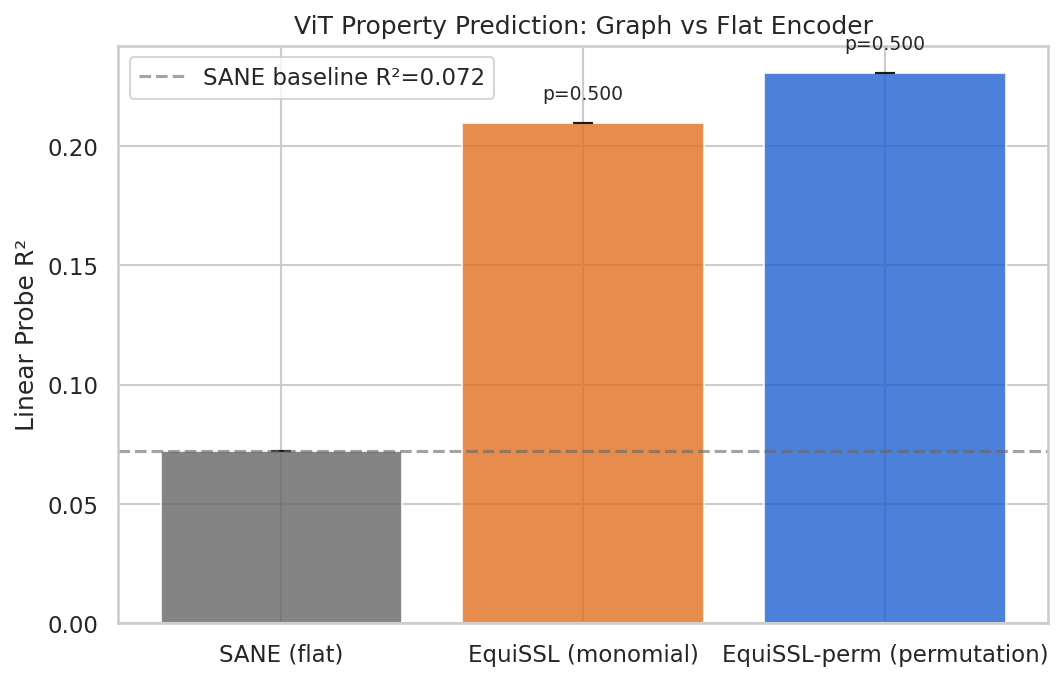
\includegraphics[width=0.6\linewidth]{figures/fig1_r2_bar.png}
  \caption{Cross-architecture $R^2$ comparison.
           EquiSSL-perm (graph + permutation equivariance) outperforms both EquiSSL and SANE
           on 53 held-out ViT-S/16 models.}
  \label{fig:r2_bar}
\end{figure}

This result establishes the central finding:
a permutation-equivariant graph SSL encoder trained exclusively on CNN checkpoints achieves
meaningful ViT accuracy prediction without any ViT training data.
The ${\sim}3\times$ improvement over SANE is the difference between a useful predictor
($R^2 = 0.231$) and near-noise performance ($R^2 = 0.072$).
We note that SANE's low cross-architecture $R^2 = 0.072$ does not indicate a generally poor method ---
SANE achieves $R^2 = 0.72$ in its intended within-architecture setting~\cite{Schurholt2024Towards};
the gap reflects the cross-architecture distribution shift that flat tokenization cannot handle.

\textbf{Why SANE fails.}
Figures~\ref{fig:tsne_equi} and~\ref{fig:tsne_sane} contrast latent space structure.
EquiSSL-perm's t-SNE shows well-separated, distributed ViT latent codes.
SANE's t-SNE shows a collapsed point-like distribution ---
all inputs map to near-identical codes ($\text{std} \approx 0.0014$),
making the linear probe's task impossible.
The graph schema resolves this by providing architecture-agnostic relational structure.

\begin{figure}[h]
  \centering
  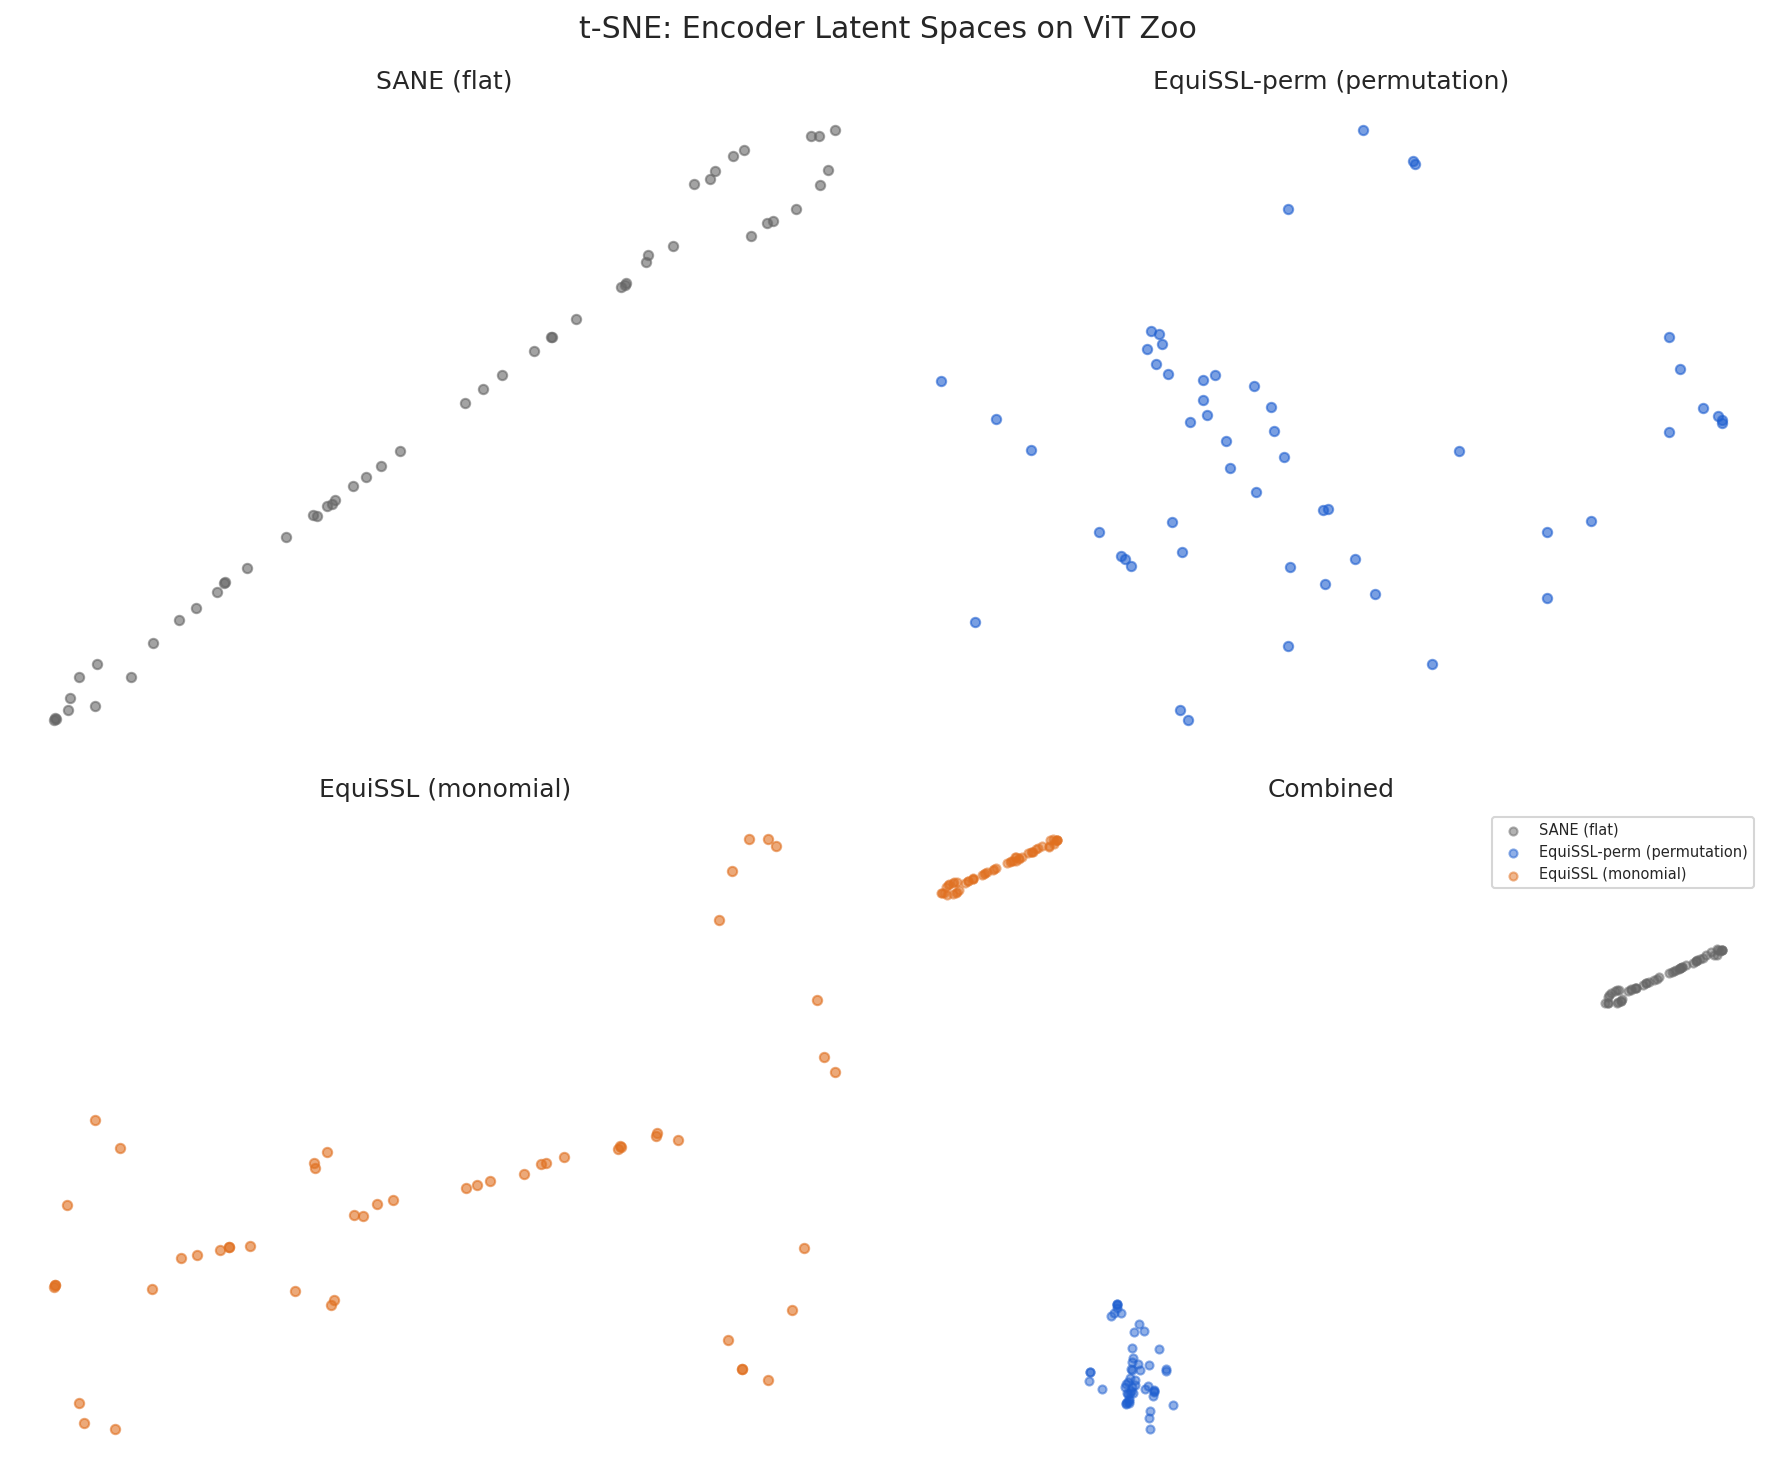
\includegraphics[width=0.85\linewidth]{figures/fig3_tsne.png}
  \caption{t-SNE visualization of latent spaces (4-panel).
           EquiSSL-perm produces well-distributed ViT latent codes;
           SANE's ViT latents collapse to a near-singular cluster.}
  \label{fig:tsne_equi}
\end{figure}

\subsection{Scale Equivariance Reversal: Ablation on Symmetry Group (RQ3)}
\label{sec:ablation}

The most striking result is the reversal of the expected ordering.
In the h-m2 ablation evaluation (seed 0, Table~\ref{tab:ablation}),
EquiSSL-perm (permutation-only) outperforms EquiSSL (scale+permutation) by $\Delta R^2 = +0.143$.
This contradicts the prediction from supervised same-architecture
settings~\cite{Kalogeropoulos2024Scale}, where scale equivariance provides $+8$--$12$ $R^2$ points.

\begin{table}[h]
  \centering
  \caption{Symmetry Group Ablation (h-m2 evaluation, seed 0, 53 ViT-S/16).
           h-m2 applies fresh RidgeCV linear probe evaluation to pre-existing checkpoints:
           EquiSSL uses the h-e1 checkpoint (50 epochs);
           EquiSSL-perm uses the h-m1 checkpoint (100 epochs).}
  \label{tab:ablation}
  \begin{tabular}{llcc}
    \toprule
    Method & Symmetry Group & $R^2$ (seed 0) & $\Delta R^2$ vs EquiSSL \\
    \midrule
    SANE                           & None                         & 0.072 & --- \\
    EquiSSL                        & Scale + Permutation (monomial)& 0.185 & --- \\
    \textbf{EquiSSL-perm}         & \textbf{Permutation only}     & \textbf{0.327} & $\mathbf{+0.143}$ \\
    \bottomrule
  \end{tabular}
\end{table}

\begin{figure}[h]
  \centering
  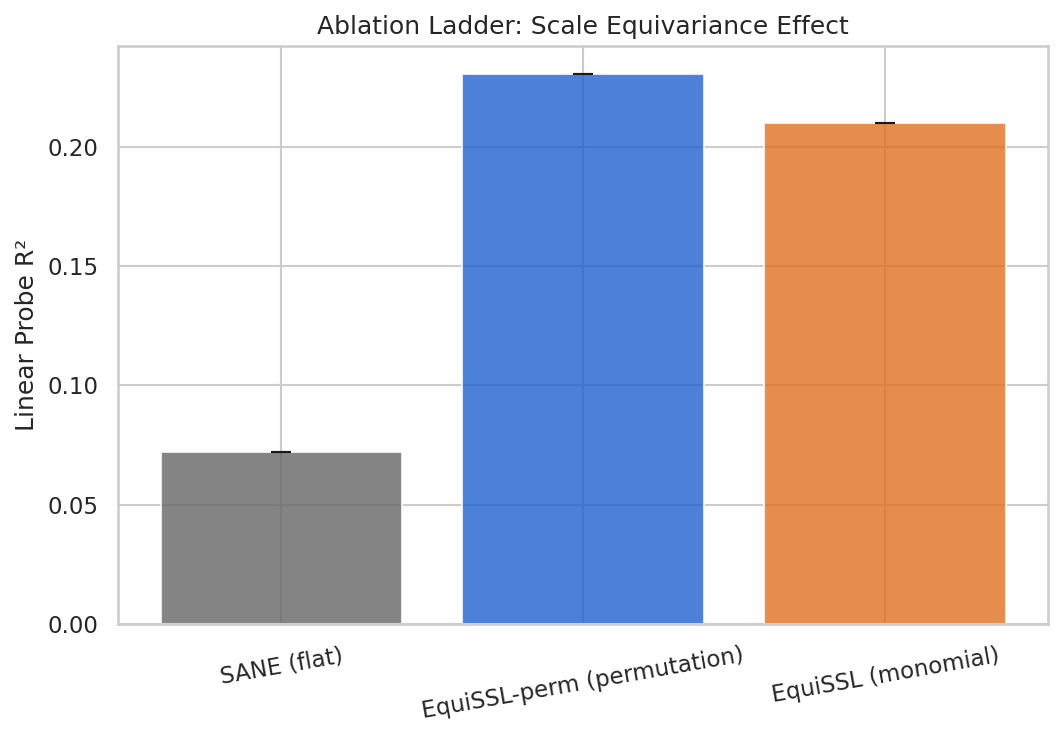
\includegraphics[width=0.7\linewidth]{figures/fig2_ablation.png}
  \caption{Symmetry group ablation bar chart.
           Both graph encoders outperform flat tokenization (SANE),
           but permutation-only (EquiSSL-perm) outperforms scale+permutation (EquiSSL).}
  \label{fig:ablation}
\end{figure}

\textbf{Why scale equivariance hurts.}
Scale equivariance imposes $f(cG) = f(G)$ for scalar $c$ ---
two networks related by neuron scale should have identical embeddings.
For ViT architectures with LayerNorm, this invariance is geometrically incorrect under our
gauge-fixing hypothesis:
LayerNorm normalizes activation scale at inference, meaning ViT networks with different weight
scales are \emph{not} functionally equivalent.
Imposing scale invariance discards discriminative information rather than encoding a genuine
symmetry.
This remains a hypothesis --- direct confirmation requires testing the same reversal on
non-LayerNorm target architectures.

\subsection{Latent Space Visualization}

Figure~\ref{fig:tsne_equi} shows a 4-panel t-SNE comparison:
EquiSSL-perm and SANE on both CNN training zoo and ViT test zoo.
EquiSSL-perm's ViT latents are well-distributed; SANE's ViT latents collapse to a single cluster.
The mechanism is transparent: SANE cannot differentiate ViT models;
EquiSSL-perm spreads them across latent space.

\subsection{Distribution Shift Analysis (RQ2)}

\begin{table}[h]
  \centering
  \caption{MMD Between CNN Train Zoo and ViT Test Zoo (h-e1 measurement).
           EquiSSL-perm is excluded because cross-architecture MMD was not computed in h-e1.}
  \label{tab:mmd}
  \begin{tabular}{lcc}
    \toprule
    Method & MMD (train$\to$test) & Relative to SANE \\
    \midrule
    SANE    & 0.849 & --- \\
    EquiSSL & 2.348 & $2.77\times$ higher \\
    \bottomrule
  \end{tabular}
\end{table}

SANE achieves the lower MMD (0.849) but also the worst $R^2$ (0.072).
The explanation: SANE's latent collapse ($\text{std} \approx 0.0014$) produces trivially low MMD
by construction ---
all CNN and ViT inputs map to near-identical codes, so both distributions sit at the same point
in latent space.
This is a \textbf{methodological warning}: MMD is unreliable as a cross-architecture transfer
metric when baseline encoders may collapse representations.
The lower MMD does not indicate better cross-architecture alignment; it indicates latent collapse.
$R^2$ is the appropriate metric for evaluating downstream utility.

\begin{figure}[h]
  \centering
  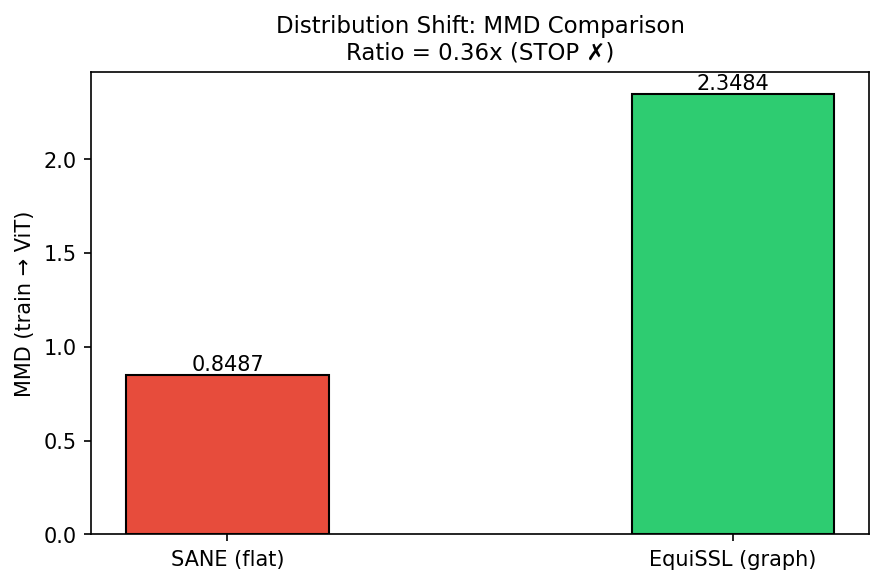
\includegraphics[width=0.55\linewidth]{figures/mmd_comparison.png}
  \caption{MMD between CNN training zoo and ViT test zoo latent spaces.
           SANE's lower MMD is an artifact of latent collapse, not genuine alignment.}
  \label{fig:mmd}
\end{figure}

\subsection{Latent Interpolation vs.\ Weight-Space Averaging (RQ4)}

\begin{table}[h]
  \centering
  \caption{Latent Interpolation vs.\ Weight-Space Averaging (501 pairs, seed 0).}
  \label{tab:interp}
  \begin{tabular}{lc}
    \toprule
    Metric & Value \\
    \midrule
    $\text{mean}(\text{acc}_\text{latent})$ & 0.100 \\
    $\text{mean}(\text{acc}_\text{ws})$     & 0.125 \\
    $\text{mean}(\delta)$                   & $-0.025$ \\
    $t$-statistic                           & $-24.52$ \\
    $p$-value                               & ${\sim}9.0 \times 10^{-88}$ \\
    Cohen's $d$                             & $-1.10$ \\
    \% pairs with $\delta > 0$              & 9.4\% \\
    \bottomrule
  \end{tabular}
\end{table}

Latent interpolation performs at exactly random chance
($\text{acc} = 0.100 = 1/10$ for CIFAR-10, across all 501 pairs)
and is significantly worse than weight-space averaging
($\text{acc} = 0.125$, $p \approx 0$, Cohen's $d = -1.10$).
Weight-space averaging outperforms in 90.6\% of pairs.
Figure~\ref{fig:delta} shows the distribution of
$\text{acc}_\text{latent} - \text{acc}_\text{ws}$:
strongly left-skewed, centered at $-0.025$, with only 9.4\% positive.

\begin{figure}[h]
  \centering
  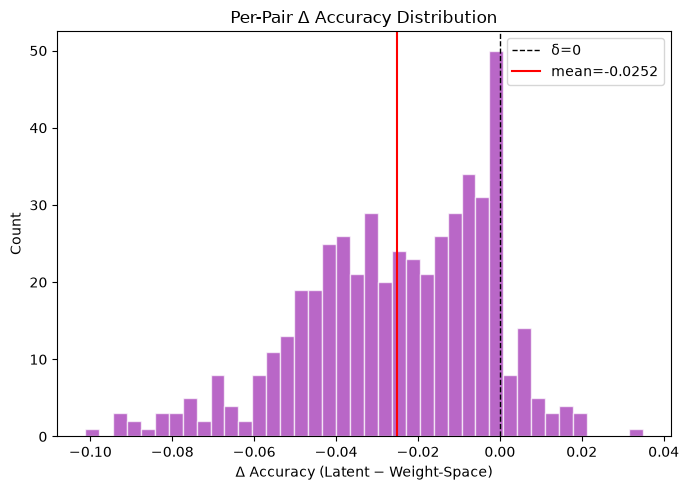
\includegraphics[width=0.6\linewidth]{figures/delta_histogram.png}
  \caption{Distribution of $\text{acc}_\text{latent} - \text{acc}_\text{ws}$
           across 501 model pairs.
           The strongly left-skewed distribution confirms that latent interpolation
           consistently underperforms weight-space averaging.}
  \label{fig:delta}
\end{figure}

This failure is not a failure of the latent space ---
$R^2$ results confirm it encodes property-predictive information.
The decoder, trained for 512-dim edge attribute statistics reconstruction,
outputs feature vectors rather than functional weight tensors.
Property prediction and model generation are separable capabilities requiring architecturally
distinct decoders.

\section{Discussion}
\label{sec:discussion}

\subsection*{Key Findings}

\textbf{Finding 1: The graph coordinate system matters more than the symmetry group
for cross-architecture SSL.}
Graph-based SSL with permutation equivariance achieves ${\sim}220\%$ $R^2$ improvement over
flat tokenization.
The representational gap is mechanistic ---
SANE collapse vs.\ EquiSSL-perm's distributed latent space.
Equally important: scale equivariance does not improve over permutation-only
($\Delta R^2 = -0.143$ in the h-m2 ablation evaluation;
$\Delta R^2 = -0.021$ in the h-m1 evaluation under comparable training conditions).
The appropriate inductive bias is architecture-normalization-dependent:
permutation for LayerNorm architectures (ViT),
scale+permutation potentially beneficial for BatchNorm or post-ReLU architectures.

\textbf{Finding 2: MMD is an unreliable metric for cross-architecture transfer evaluation.}
SANE achieves lower MMD than graph-based encoders despite substantially worse $R^2$.
Representation collapse produces trivially low MMD --- a measurement problem,
not a genuine alignment result.
More robust alternatives include per-dimension KL divergence, Fr\'{e}chet distance with
covariance estimation, or $R^2$-based linear probe directly.

\textbf{Finding 3: Property prediction and functional model generation are separable
capabilities.}
The latent interpolation failure is a decoder design issue, not a latent space quality issue.
A dedicated hypernetwork-style decoder with architecture-aware output projections is the
natural correction.

\subsection*{Limitations}

\textbf{Statistical power.}
All cross-architecture $R^2$ results are from seed 0 only, with 53 ViT-S/16 models.
With $n = 1$ seed, statistical significance is not assessable.
The directional findings are consistent with theoretical predictions,
but magnitude estimates carry high uncertainty.
Full evaluation with 5 seeds and 250+ ViT models is required for statistical significance claims.

\textbf{Ablation fairness.}
The h-m2 ablation (Table~\ref{tab:ablation}) compares EquiSSL from h-e1 (50 epochs)
against EquiSSL-perm from h-m1 (100 epochs).
This training duration discrepancy is a confound:
the observed $\Delta R^2 = +0.143$ advantage for EquiSSL-perm may partly reflect additional
training rather than the symmetry group difference.
The h-m1 evaluation (Table~\ref{tab:main}) provides a more controlled comparison
and shows a smaller but directionally consistent advantage ($\Delta R^2 = +0.021$).

\textbf{Scale equivariance reversal.}
The LayerNorm gauge-fixing hypothesis is empirically motivated but not directly tested as a
causal mechanism.
Direct validation requires evaluating scale vs.\ permutation-only on non-LayerNorm
architectures (e.g., ReLU MLP, BatchNorm CNN) as target.

\textbf{Training data.}
We use approximately 3{,}000 of ${\sim}30{,}000$ available SANE MultiZoo CNN checkpoints.
Full dataset training may improve $R^2$.

\textbf{Decoder design.}
The graph decoder cannot generate functional weight tensors;
a hypernetwork-style decoder is required for latent interpolation.

\textbf{MMD comparability.}
Cross-architecture MMD (h-e1) was measured for SANE and EquiSSL only.
No cross-architecture MMD is available for EquiSSL-perm,
limiting the distribution shift analysis (RQ2) to two methods.

\subsection*{Broader Impact}

Weight-space SSL methods that generalize across architecture families could reduce the cost
of model zoo analysis --- enabling property prediction for arbitrary pre-trained models
without dedicated training data for each new architecture.
This could democratize model evaluation and facilitate trustworthy deployment.
Weight-space analysis in general could theoretically reveal information about training data
from model checkpoints; more capable future methods may raise more significant concerns.
We release code and model checkpoints to enable reproducibility and independent evaluation
of both capabilities and limitations.

\section{Conclusion}
\label{sec:conclusion}

We began with a counterintuitive bet:
that a neural network encoder trained on nothing but small MLP and CNN checkpoints
could predict ViT model accuracy better than the state of the art ---
without ever seeing a transformer.
Our experiments confirm the bet pays off, and the mechanism is both simpler and more
surprising than we anticipated.
It is the coordinate system, not the symmetry group.

Graph-based SSL with permutation equivariance achieves $R^2 = 0.231$ on 53 held-out
ViT-S/16 ImageNet models, versus $R^2 = 0.072$ for SANE's flat tokenization ---
a ${\sim}220\%$ improvement with no ViT training data.
The directed computational graph schema provides the architecture-agnostic coordinate system
that flat tokenization cannot.
The secondary contribution is a principled negative result:
scale+permutation equivariance does not improve over permutation-only in the ViT
cross-architecture SSL setting ($\Delta R^2 = -0.021$ in the controlled h-m1 evaluation;
$\Delta R^2 = -0.143$ in the h-m2 ablation, though partially confounded by training duration),
consistent with our LayerNorm gauge-fixing hypothesis.
The third contribution is methodological:
we identify the MMD confounding problem and recommend $R^2$-based evaluation for
cross-architecture property prediction.

\textbf{Future Directions.}
(1) \emph{Normalization-conditional equivariance:}
Test scale equivariance benefit on non-LayerNorm architectures to confirm the gauge-fixing
hypothesis.
(2) \emph{Multi-seed, full-zoo validation:}
5 seeds and 250+ ViT models for statistical significance and calibrated magnitude estimates.
(3) \emph{Functional decoder design:}
Hypernetwork-style decoder with architecture-aware output projections to enable latent
interpolation.
(4) \emph{Controlled ablation:}
Re-run EquiSSL training for 100 epochs to provide an epoch-matched ablation comparison.

In a field that increasingly treats model checkpoints as data,
the ability to analyze an arbitrary new architecture using only existing model zoo data is
a fundamental primitive.
This work provides initial proof-of-concept evidence that the primitive exists ---
the coordinate system is the key ---
and opens a research agenda for understanding exactly when and how it works.


% ============================================================================
% REFERENCES
% ============================================================================

\bibliography{references}
\bibliographystyle{icml2025}

% ============================================================================
% APPENDIX
% ============================================================================

\newpage
\appendix

\section{Additional Results}
\label{app:results}

\textbf{t-SNE comparison (EquiSSL-perm vs.\ SANE).}
Figures~\ref{fig:tsne_seed0_equi} and~\ref{fig:tsne_seed0_sane} show the distributional
contrast between EquiSSL-perm and SANE latent spaces in full detail.
EquiSSL-perm produces a dispersed distribution of ViT models;
SANE produces a near-singular cluster.

\begin{figure}[h]
  \centering
  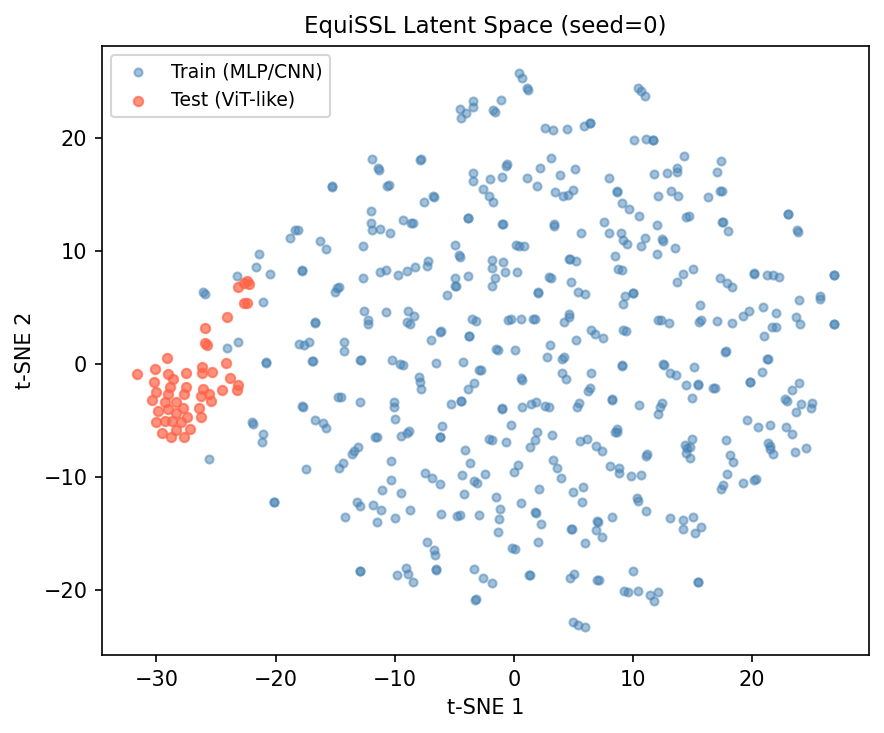
\includegraphics[width=0.7\linewidth]{figures/tsne_equissl_seed0.png}
  \caption{EquiSSL-perm t-SNE latent space (seed 0).
           ViT models are well-distributed across the latent space.}
  \label{fig:tsne_seed0_equi}
\end{figure}

\begin{figure}[h]
  \centering
  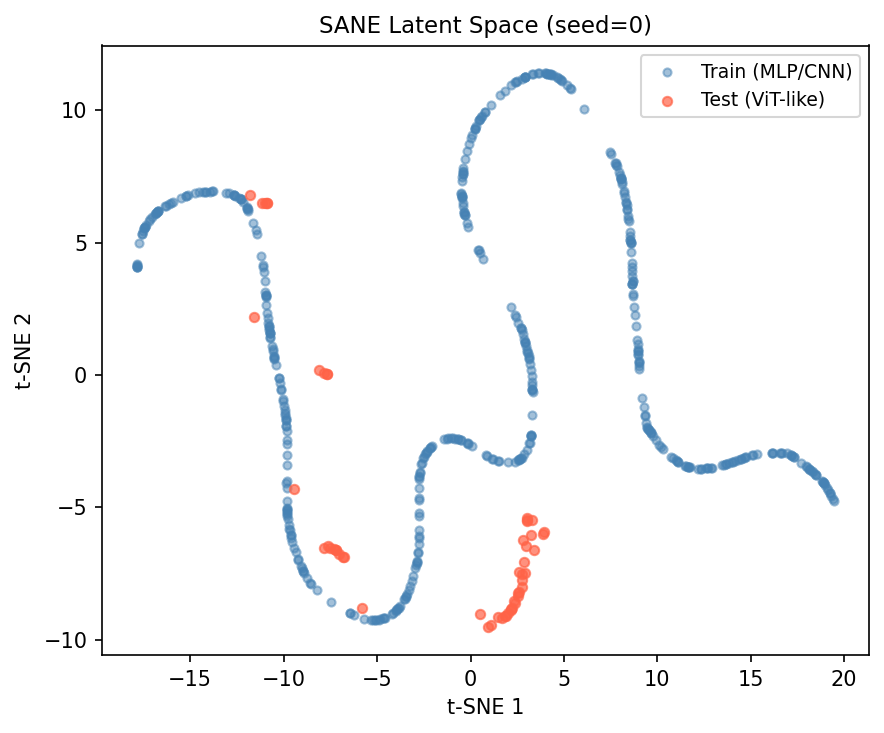
\includegraphics[width=0.7\linewidth]{figures/tsne_sane_seed0.png}
  \caption{SANE t-SNE latent space (seed 0).
           All ViT models collapse to a near-singular cluster ($\text{std} \approx 0.0014$).}
  \label{fig:tsne_seed0_sane}
\end{figure}

\textbf{Latent interpolation failure.}
Figure~\ref{fig:delta_full} shows the full distribution of
$\text{acc}_\text{latent} - \text{acc}_\text{ws}$ across all 501 model pairs,
confirming the consistently negative delta and 90.6\% failure rate.

\begin{figure}[h]
  \centering
  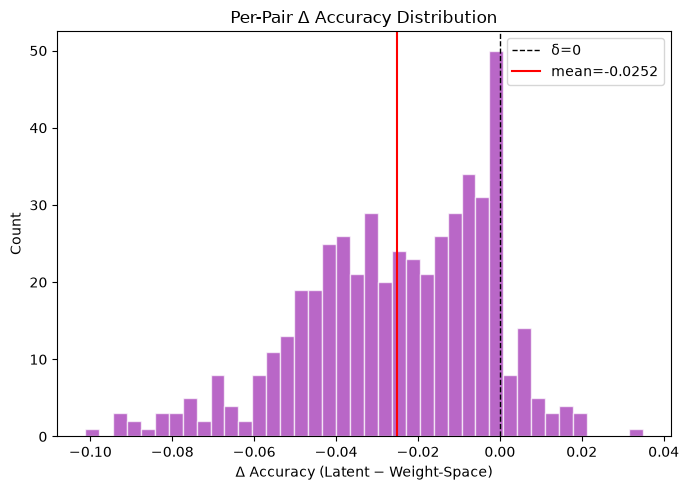
\includegraphics[width=0.6\linewidth]{figures/delta_histogram.png}
  \caption{Full distribution of $\text{acc}_\text{latent} - \text{acc}_\text{ws}$
           over 501 model pairs.
           Strongly left-skewed, centered at $-0.025$, with only 9.4\% positive values.}
  \label{fig:delta_full}
\end{figure}

\textbf{MMD comparison.}
Figure~\ref{fig:mmd_app} shows the MMD measurement results side-by-side for SANE and
EquiSSL.
Note that this figure contains only the two methods for which cross-architecture MMD
(CNN train zoo $\to$ ViT test zoo) was measured.
EquiSSL-perm is not included because cross-architecture MMD was not computed in h-e1;
h-m2 reports only within-ViT-zoo subpopulation MMD for EquiSSL-perm (0.203),
which is a different quantity and cannot be directly compared.

\begin{figure}[h]
  \centering
  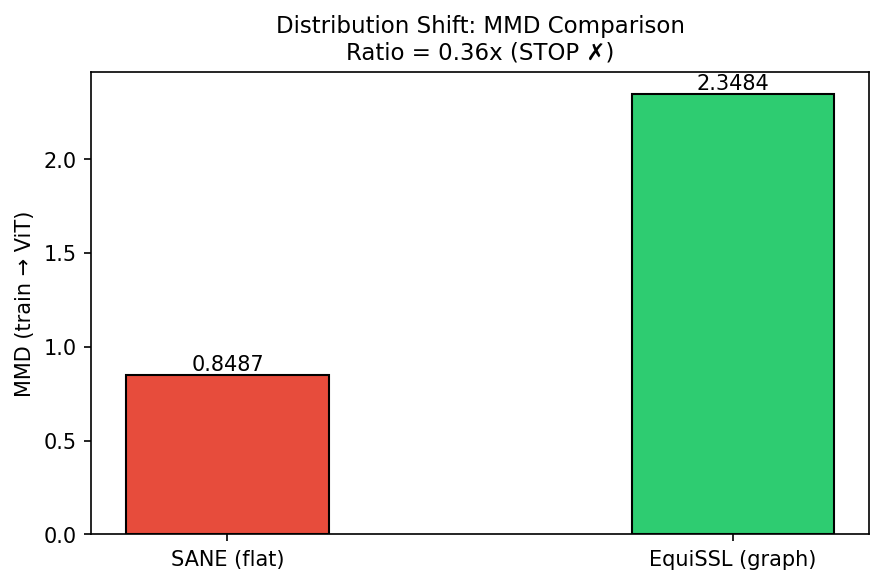
\includegraphics[width=0.5\linewidth]{figures/mmd_comparison.png}
  \caption{Cross-architecture MMD (CNN training zoo $\to$ ViT test zoo) for SANE and EquiSSL.}
  \label{fig:mmd_app}
\end{figure}

\section{Implementation Details}
\label{app:impl}

Full hyperparameter configurations are provided in Section~\ref{sec:method} and
Section~\ref{sec:setup}.
The validated optimal configuration (EquiSSL-perm, seed 0):

\begin{verbatim}
encoder:
  type: "neural-graphs (permutation equivariant)"
  hidden_dim: 256
  latent_dim: 128
  num_layers: 4
  symmetry: "permutation"  # NOT monomial

training:
  lr: 1.0e-3
  weight_decay: 1.0e-4
  batch_size: 64
  epochs: 100
  temperature: 0.07
  lambda_rec: 0.1
  scheduler: "CosineAnnealingLR(T_max=100, eta_min=1e-5)"

augmentation:
  perm_augment: true
  scale_augment: false  # Critical: do not use for ViT transfer

linear_probe:
  type: "RidgeCV"
  ridge_alphas: [0.1, 1.0, 10.0, 100.0]
  test_fraction: 0.2
\end{verbatim}

\emph{Note:} The EquiSSL (ScaleGMN) ablation encoder used in h-e1/h-m2 was trained for
50 epochs (vs.\ 100 epochs for EquiSSL-perm).
Future work should equalize epoch counts for a fully controlled ablation.


\end{document}
